% =====================================================================
% MSc thesis defense slides
% Does implied volatility efficiently predict future realized volatility,
% and how does this relationship vary across market regimes and between
% cryptocurrency and equity markets?
% Gabin Torres and Clement Massabo - SKEMA Business School - May 2025
% =====================================================================
\documentclass[aspectratio=169,11pt]{beamer}

% ---------- Fonts ----------
\usepackage[T1]{fontenc}
\usepackage[utf8]{inputenc}
\usepackage{libertinus-type1}   % serif Libertinus
\usepackage{microtype}

% ---------- Math, tables, graphics ----------
\usepackage{amsmath,amssymb}
\usepackage{booktabs}
\usepackage{array}
\usepackage{graphicx}
\usepackage{tikz}

% ---------- Colours ----------
\usepackage{xcolor}
\definecolor{navy}{HTML}{1F4E79}
\definecolor{charcoal}{HTML}{1F2937}
\definecolor{lightgrey}{HTML}{E5E7EB}
\definecolor{midgrey}{HTML}{6B7280}

% ---------- Beamer theme: sober custom ----------
\usetheme{default}
\useinnertheme{rectangles}
\useoutertheme{default}
\setbeamercolor{normal text}{fg=charcoal,bg=white}
\setbeamercolor{title}{fg=navy}
\setbeamercolor{frametitle}{fg=navy}
\setbeamercolor{structure}{fg=navy}
\setbeamercolor{block title}{fg=navy,bg=lightgrey}
\setbeamercolor{block body}{fg=charcoal,bg=white}
\setbeamerfont{title}{series=\bfseries,size=\Large,family=\sffamily}
\setbeamerfont{frametitle}{series=\bfseries,size=\large,family=\sffamily}
\setbeamerfont{author}{size=\normalsize}
\setbeamerfont{date}{size=\small}
\setbeamerfont{footline}{size=\tiny}

% No navigation symbols, clean footline
\setbeamertemplate{navigation symbols}{}
\setbeamertemplate{footline}{%
  \hfill\textcolor{midgrey}{\tiny G.~Torres \& C.~Massabo \,$\cdot$\, MSc FMI \,$\cdot$\, May 2025 \quad
  \insertframenumber/\inserttotalframenumber}\hspace*{4mm}\vspace*{3mm}}

% Custom frame title with a navy rule beneath
\setbeamertemplate{frametitle}{%
  \nointerlineskip\vspace*{4mm}%
  \begin{beamercolorbox}[wd=\paperwidth,leftskip=8mm,rightskip=8mm]{frametitle}%
    \usebeamerfont{frametitle}\insertframetitle\par%
    \vspace*{1.5mm}\textcolor{navy}{\rule{\dimexpr\paperwidth-16mm\relax}{0.6pt}}%
  \end{beamercolorbox}%
}

% Item bullets: small navy squares
\setbeamertemplate{itemize item}{\textcolor{navy}{\rule[0.4ex]{1.4ex}{1.4ex}}}
\setbeamertemplate{itemize subitem}{\textcolor{navy}{\rule[0.4ex]{1.0ex}{1.0ex}}}

% No section bars
\setbeamertemplate{section in toc}[default]

% Hyperref (already loaded by beamer; just configure)
\hypersetup{colorlinks=true,linkcolor=navy,urlcolor=navy,citecolor=navy}
\usepackage{url}

% =====================================================================
% TITLE INFO
% =====================================================================
\title{Does implied volatility efficiently predict future realized volatility?}
\subtitle{And how does the answer differ between Bitcoin and the S\&P~500?}
\author{Gabin Torres \and Cl\'ement Massabo}
\institute{MSc Financial Markets \& Investments \\ SKEMA Business School}
\date{May 2025}

\begin{document}

% =====================================================================
% SLIDE 1 - COVER
% =====================================================================
\begin{frame}[plain]
  \vspace*{4mm}
  \begin{center}
    {\Large\sffamily\bfseries\color{navy}
      Does implied volatility efficiently predict\\[2pt]
      future realized volatility?\par}
    \vspace*{4mm}
    {\normalsize\itshape And how does the answer differ between\\
      Bitcoin and the S\&P~500?\par}
    \vspace*{12mm}
    \textcolor{navy}{\rule{0.6\textwidth}{0.6pt}}
    \vspace*{6mm}

    {\large\bfseries Gabin Torres \quad \&\quad Cl\'ement Massabo\par}
    \vspace*{4mm}
    {\small\itshape Thesis Supervisor: Alexandre Landi\par}
    \vspace*{10mm}
    {\small MSc Financial Markets \& Investments\par}
    {\small SKEMA Business School, May 2025\par}
  \end{center}
\end{frame}

% =====================================================================
% SLIDE 2 - RESEARCH QUESTION
% =====================================================================
\begin{frame}{The research question}
  \vspace*{6mm}
  \begin{center}
    {\Large\bfseries\color{navy}
      Does implied volatility predict future realized volatility?\par}
    \vspace*{3mm}
    {\large\itshape Same answer for Bitcoin and the S\&P~500?\par}
  \end{center}
  \vspace*{8mm}
  \begin{itemize}
    \item Implied volatility is the market's forecast of future risk.
    \item In equities, the relationship has been studied for thirty years.
    \item In crypto, it has barely been documented.
  \end{itemize}
\end{frame}

% =====================================================================
% SLIDE 3 - LIT REVIEW + GAP
% =====================================================================
\begin{frame}{What we know vs. what we don't}
  \vspace*{2mm}
  \begin{columns}[T,onlytextwidth]
    \column{0.48\textwidth}
    \begin{block}{Equity markets}
      \begin{itemize}
        \setlength\itemsep{2mm}
        \item Implied volatility is informative \\
          {\footnotesize Christensen \& Prabhala (1998)}
        \item Slope below one, positive premium \\
          {\footnotesize Bollerslev, Tauchen \& Zhou (2009)}
        \item Predictive power weakens in crises \\
          {\footnotesize Whaley (2009), Giot (2005)}
      \end{itemize}
    \end{block}
    \column{0.48\textwidth}
    \begin{block}{Crypto markets}
      \begin{itemize}
        \setlength\itemsep{2mm}
        \item DVOL exists only since March 2021
        \item No published predictive evidence
        \item No regime-conditional analysis of BTC option markets
      \end{itemize}
    \end{block}
  \end{columns}
  \vspace*{4mm}
  \begin{center}
    \textcolor{navy}{\itshape Our contribution: apply the equity benchmark to crypto, in a unified framework, with regime splits.}
  \end{center}
\end{frame}

% =====================================================================
% SLIDE 4 - HYPOTHESES
% =====================================================================
\begin{frame}{Five hypotheses}
  \vspace*{3mm}
  \begin{itemize}
    \setlength\itemsep{3mm}
    \item \textbf{H1.}~Implied volatility overestimates future realized volatility on average: positive variance risk premium.
    \item \textbf{H2.}~Implied volatility is informative but not a perfect predictor.
    \item \textbf{H3.}~The variance risk premium is larger in crypto than in equities.
    \item \textbf{H4.}~The predictive relationship weakens in stress periods.
    \item \textbf{H5.}~Equity markets are close to efficient in normal periods; crypto is not.
  \end{itemize}
\end{frame}

% =====================================================================
% SLIDE 5 - DATA
% =====================================================================
\begin{frame}{Data}
  \vspace*{3mm}
  \begin{center}
    \small
    \begin{tabular}{lll}
      \toprule
      Series & Provider & Identifier \\
      \midrule
      Bitcoin spot          & Binance public API       & \texttt{BTCUSDT} daily \\
      Bitcoin implied vol.  & Deribit public API       & \texttt{BTC\_DVOL} \\
      S\&P 500 close        & Yahoo Finance (\texttt{yfinance}) & \texttt{\^{}GSPC} \\
      VIX close             & Yahoo Finance (\texttt{yfinance}) & \texttt{\^{}VIX} \\
      \bottomrule
    \end{tabular}
  \end{center}
  \vspace*{6mm}
  \begin{itemize}
    \item \textbf{Period:} 24 March 2021 \,$\to$\, 31 December 2025.
    \item \textbf{After NYSE-calendar inner join:} 1\,201 daily observations.
    \item All series come from public APIs (no proprietary terminal data).
  \end{itemize}
\end{frame}

% =====================================================================
% SLIDE 6 - METHOD
% =====================================================================
\begin{frame}{Method, in one slide}
  \vspace*{3mm}
  \begin{itemize}
    \setlength\itemsep{3.5mm}
    \item \textbf{Realized volatility:} annualised standard deviation of 30-day log returns.
    \item \textbf{Predictive regression:} future realized volatility regressed on current implied volatility.
      \\[1pt]
      {\itshape Slope $= 1$ means efficient.}
    \item \textbf{Regimes:} \textit{stress} $=$ top 10\,\% of VIX (equities) or BTC realized volatility (crypto), set ex~ante.
    \item \textbf{Inference:} Newey--West HAC standard errors to correct for rolling-window overlap.
  \end{itemize}
\end{frame}

% =====================================================================
% SLIDE 7a - FIRST LOOK: BITCOIN (TRANSITION)
% =====================================================================
\begin{frame}{A first look: Bitcoin}
  \vspace*{3mm}
  \begin{center}
    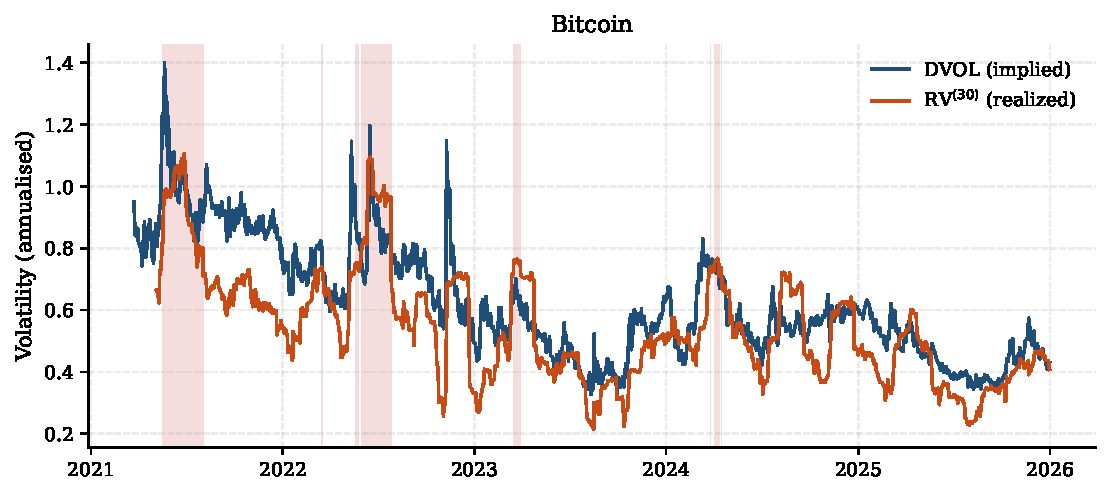
\includegraphics[width=0.88\textwidth]{../media/fig_iv_rv_timeline_btc.pdf}
  \end{center}
  \vspace*{3mm}
  \begin{itemize}
    \item DVOL and 30-day realized volatility move together, with a positive average wedge.
    \item Red shading: stress days (BTC 30-day RV above its 90th percentile, set ex~ante).
  \end{itemize}
\end{frame}

% =====================================================================
% SLIDE 7b - FIRST LOOK: S&P 500
% =====================================================================
\begin{frame}{A first look: S\&P~500}
  \vspace*{3mm}
  \begin{center}
    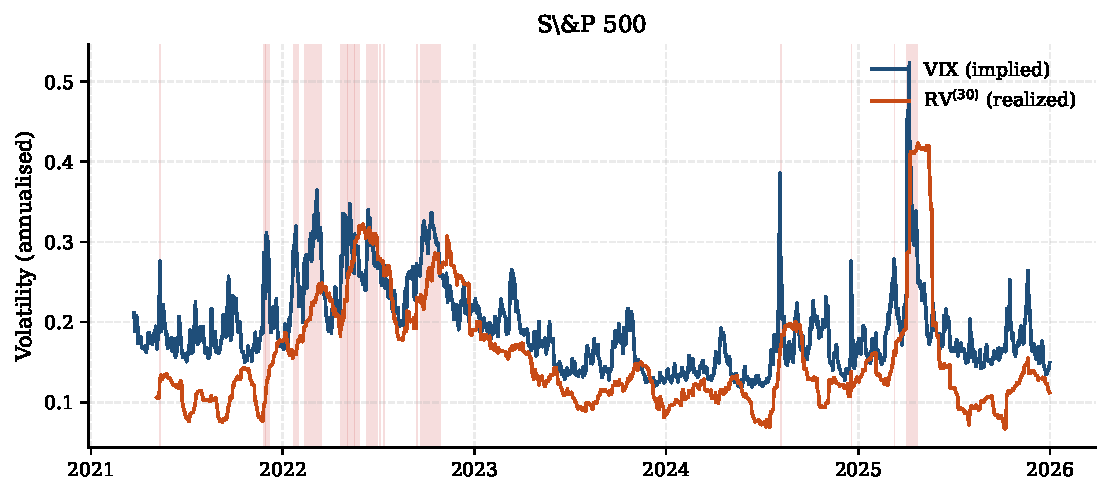
\includegraphics[width=0.88\textwidth]{../media/fig_iv_rv_timeline_spx.pdf}
  \end{center}
  \vspace*{3mm}
  \begin{itemize}
    \item Volatility runs in a much narrower band than Bitcoin, but spikes sharply in crises.
    \item Red shading: stress days (VIX above its 90th percentile, set ex~ante).
  \end{itemize}
\end{frame}

% =====================================================================
% SLIDE 8 - RESULT 1: GLOBAL REGRESSIONS
% =====================================================================
\begin{frame}{Implied volatility is informative, but biased}
  \vspace*{4mm}
  \begin{center}
    \small
    \renewcommand{\arraystretch}{1.2}
    \begin{tabular}{lcc}
      \toprule
      & \textbf{Bitcoin} & \textbf{S\&P 500} \\
      \midrule
      Slope $\hat\beta$              & \textcolor{navy}{\textbf{0.55}}$^{***}$ & \textcolor{navy}{\textbf{0.79}}$^{***}$ \\
      HAC s.e.                       & (0.09) & (0.10) \\
      $R^2$                          & 0.33 & 0.36 \\
      $H_0: \beta = 1$               & rejected ($p<0.001$) & rejected ($p = 0.03$) \\
      $N$                            & 1\,171 & 1\,171 \\
      \bottomrule
    \end{tabular}
  \end{center}
  \vspace*{5mm}
  \begin{itemize}
    \item Both slopes are highly significant: implied volatility carries real information.
    \item Both are significantly below one: positive variance risk premium in both markets.
  \end{itemize}
  \vspace*{2mm}
  {\footnotesize\itshape $^{***}$ significant at 1\,\%. Standard errors: Newey--West HAC, 30 lags.}
\end{frame}

% =====================================================================
% SLIDE 9 - VRP COMPARISON
% =====================================================================
\begin{frame}{The variance risk premium is larger in crypto}
  \vspace*{8mm}
  \begin{center}
    \begin{tabular}{ccc}
      \textbf{Bitcoin} & & \textbf{S\&P 500} \\[2mm]
      {\fontsize{42}{50}\selectfont\color{navy}\textbf{+0.081}} & \quad vs.\ \quad &
      {\fontsize{42}{50}\selectfont\color{navy}\textbf{+0.035}} \\[2mm]
      {\small\itshape avg.\ variance risk premium} & & {\small\itshape avg.\ variance risk premium} \\
    \end{tabular}
  \end{center}
  \vspace*{8mm}
  \begin{center}
    {\itshape Crypto investors require more than twice the compensation\\
    per unit of volatility risk.}\par
    \vspace*{2mm}
    \textcolor{navy}{Confirms H3.}
  \end{center}
\end{frame}

% =====================================================================
% SLIDE 10 - HEADLINE: SPX NORMAL CLOSE TO EFFICIENT
% =====================================================================
\begin{frame}{Headline result}
  \vspace*{3mm}
  \begin{center}
    {\small\itshape In calm markets, the VIX looks almost efficient.}
  \end{center}
  \vspace*{4mm}
  \begin{center}
    {\fontsize{44}{52}\selectfont\color{navy}\textbf{$\hat\beta = 0.97$}}\\[2mm]
    {\normalsize S\&P~500, normal regime, $N = 955$}
  \end{center}
  \vspace*{6mm}
  \begin{center}
    {\large $p = 0.89$\, for\, $H_0:\beta = 1$}
  \end{center}
  \vspace*{6mm}
  \begin{center}
    \textcolor{navy}{\bfseries We cannot reject that the VIX is a fully efficient predictor\\
    of S\&P~500 realized volatility in normal periods.}
  \end{center}
\end{frame}

% =====================================================================
% SLIDE 11 - VRP ASYMMETRY IN STRESS
% =====================================================================
\begin{frame}{The premium reacts to stress in opposite directions}
  \vspace*{4mm}
  \begin{center}
    \small
    \renewcommand{\arraystretch}{1.3}
    \begin{tabular}{lccc}
      \toprule
      & \textbf{Normal} & \textbf{Stress} & \textbf{Direction} \\
      \midrule
      \textbf{Bitcoin}        & $+0.087$ & \textcolor{navy}{\textbf{$+0.055$}} & \textit{compresses} \\
      \textbf{S\&P 500}       & $+0.032$ & \textcolor{navy}{\textbf{$+0.047$}} & \textit{widens} \\
      \bottomrule
    \end{tabular}
  \end{center}
  \vspace*{5mm}
  \begin{itemize}
    \item \textbf{Equity stress} $\Rightarrow$ premium \textit{widens}. Implied volatility surges with hedging demand.
    \item \textbf{Crypto stress} $\Rightarrow$ premium \textit{compresses}. Realized volatility catches up faster than DVOL.
  \end{itemize}
  \vspace*{3mm}
  \begin{center}
    \textcolor{navy}{\itshape An asymmetry only visible when both markets are studied together.}
  \end{center}
\end{frame}

% =====================================================================
% SLIDE 12 - ECONOMIC MECHANISMS
% =====================================================================
\begin{frame}{Why? Three economic mechanisms}
  \vspace*{3mm}
  \begin{enumerate}
    \setlength\itemsep{4mm}
    \item \textbf{Hedging demand.} Equity investors buy out-of-the-money puts in stress, which pushes the VIX above expected realized volatility.
    \item \textbf{24/7 trading.} Bitcoin realized volatility adjusts to news within hours, not days, which compresses the wedge faster.
    \item \textbf{Market maturity.} Equity option markets are deep and dominated by institutions; crypto options are concentrated on a few venues and a more retail base.
  \end{enumerate}
\end{frame}

% =====================================================================
% SLIDE 13 - LIMITATIONS
% =====================================================================
\begin{frame}{What we don't claim}
  \vspace*{3mm}
  \begin{itemize}
    \setlength\itemsep{3.5mm}
    \item \textbf{Short sample.} DVOL only goes back to March 2021.
    \item \textbf{Aggregated indices.} No full option surface, so no skew and no term structure.
    \item \textbf{Daily frequency.} Intraday data would refine realized volatility.
    \item \textbf{Asymmetric regime definition.} VIX for equity stress vs.\ realized volatility for crypto stress.
  \end{itemize}
\end{frame}

% =====================================================================
% SLIDE 14 - TAKE-AWAYS
% =====================================================================
\begin{frame}{Take-aways}
  \vspace*{3mm}
  \begin{enumerate}
    \setlength\itemsep{4mm}
    \item Implied volatility is a \textbf{risk-adjusted expectation}, not a raw forecast, in both markets.
    \item Equity markets are \textbf{close to efficient in normal periods}; crypto markets are \textbf{not}.
    \item The variance risk premium \textbf{widens in equity stress} and \textbf{compresses in crypto stress}. This asymmetry is only visible across markets.
  \end{enumerate}
  \vspace*{8mm}
  \begin{center}
    \small Code, data and full pipeline:\\
    \href{https://github.com/X9ClementX9/iv-rv-thesis}{\texttt{github.com/X9ClementX9/iv-rv-thesis}}
  \end{center}
\end{frame}

% =====================================================================
% SLIDE 15 - THANK YOU
% =====================================================================
\begin{frame}[plain]
  \vspace*{6mm}
  \begin{center}
    {\fontsize{28}{34}\selectfont\sffamily\bfseries\color{navy}Thank you.}\\[2mm]
    {\normalsize\itshape Questions?}
  \end{center}
  \vspace*{8mm}
  \begin{center}
    
\includegraphics[width=20mm]{../media/qr_repo.png}\\[2mm]
    {\footnotesize\bfseries Replication materials}\\[0.5mm]
    {\footnotesize\href{https://github.com/X9ClementX9/iv-rv-thesis}{\texttt{github.com/X9ClementX9/iv-rv-thesis}}}
  \end{center}
\end{frame}

\end{document}
